\documentclass[12pt, fullpage,letterpaper]{article}
\usepackage[margin=1in]{geometry}
\usepackage{graphicx}
\title{CS6630 Visualization Fall 2017 Project \\ A Mirror of History}
\author{Yanqing Peng, Yuwei Wang}
\begin{document}
\maketitle
The title \textbf{A mirror of history} comes from the epitaph of Wei Zhen,
a famous Chinese historian:

\emph{``Using copper as a mirror allows one to keep his clothes neat. Using
history as a mirror allows one to see the future trends. Using a person as a
mirror allows one to see what is right and what is wrong.''}

\section{Basic Information}
\paragraph{Title} A Mirror of History
\paragraph{Group members}
\begin{itemize}
    \item Yanqing Peng, u1076076, yq.peng@utah.edu
    \item Yuwei Wang, u1140944, yuwei.utah@gmail.com
\end{itemize}
\paragraph{Github link} https://github.com/uvril/VisProject

\section{Background and Motivation}

History is always fascinating.  It's important to learn lessons from the past,
by understanding the causality behind historical events.  To learn about
history is to learn about humanity, which basically means developing an
understanding of ourselves.  Therefore, knowledge of history helps us prepare
better for future.

However, it can be boring to learn history by texts and numbers. We can know
from textbook that the British Empire used to rule 35,500,000 km$^2$ area of
land. But how large is it?  Showing a map of British Empire is much more
interesting than just telling the number.  Similarly, we know that the economy
of both Japan and Singapore grow dramatically after World War II, but both slow
down in 1990s.  How can we present a comparison between the economy development
of Japan and Singapore?  Showing the GDP table will be boring and hard to
understand.  Instead, showing a line chart for the GDP of Japan and Singapore
is much clearer. Therefore, visualization is essential for learning history.

Our textbooks already contain plenty of figures to visualize history. However,
it's not enough. While learning history, people have different focuses.  Alice
is interested in the border of British Empire in 1913, while Bob wants to see a
map of French colonies in 1908. Charlie would like to know the comparison
between Japan and Singapore, while Eve is curious about the comparison between
India and Pakistan.  Only with interactive visualizations can one develop the
knowledge of history with her own interests.

In this project, our goal was to make a deeper insight into history that will help
students and others who are interested in history to explore and learn about how countries
have changed over time) as well as comparison among countries in different dimensions, by constructing
an interactive visualization on history.

\section{Related Work}
When searching for project ideas, we found that there are some good
visualizations for history already, such as Delicious Visual Map of
History,
World Population
History,
Histography and so on. However, plenty of them focuses
on different aspects (e.g history events, population, empires) of history so it
is difficult for users to get an overview.  What's more, some of them are even
static, which means users can not interact with the graph. 
Among the visualizations, Chronas did the best job. It includes many aspects
and also animations on the process of history over years.
However it only focuses on displaying the overviews, without showing any analysis on each single country.
Besides, some visualizations are too complicated to be understood. Therefore, we think
making a interactive and general visualization on history is crucial.


\section{Visualization Objectives}
The main objective of this project is to interactively visualize the current situation of the world,
as well as the historical rise and fall. Our visualization is able to show the following results:

\begin{itemize}

    \item Show the historical world map at a specified year.

    \item Show the basic information (e.g. capital) of a specified country.

    \item Show the comparison on different aspects of a specified country.

    \item Show the religious composition of a specified country.

    \item Show the rankings of some statistics of a specified country.

    \item Show the population/GDP/religion distribution of the world.

    \item Show the historical statistics of a specified country.

    \item Compare the historical statistics of a set of countries.

    \item Show how historical events related to the historical statistics of a set of countries.

\end{itemize}

\section{Data and Resources}
In our project, we used a very wide range of data and resources. We spent a lot of time on data collection and processing.
    All data were processed into json format and different categories
    of data are stored in different files. For example, "pop.json" stores all population data.
    If the data file is a historical dataset, then the year attribute is the root attribute, and the country ID is the secondary attribute.
    Otherwise, the country ID is the root attribute.
In following sections, we will describe the sources of the data, and how we process the data.
\subsection{Country Indexing}
    A major challenge we encountered when processing the data was the issue of country indexing. Our dataset contained 
    formal countries that no longer exist, so we couldn't use any modern country code to index the countries.
    Moreover, there are countries that have alternative names. For example, "South Korea" and "Republic of Korea" are the same country,
    but they are used interchangeably in different datasets.
    Therefore we have to insure that they point to the same identifier.
    We tried several methods to solve this problem and 
    finally we decided to use the Wikidata id as the country index. It can uniquely represent any item that appears in Wikipedia.
    Moreover, it helped us to retrieve data from Wikidata. In our project, the Capital of a country and Head of State of a country are retrieved by Wikidata.

    We can use Wikidata queries to convert a country name to its Wikidata ID, using the following query:

        \begin{verbatim}
        SELECT ?child ?childLabel
        WHERE {
              ?child wdt:P31 wd:Q6256.
              ?child  rdfs:label ?childLabel.
              filter (lang(?childLabel) = "en").
              filter (contains(?childLabel, "COUNTRYNAME")).
        }
        \end{verbatim}

        However, for some countries that have alternative names, we had to manually build the mapping for them.

        The converted mapping is stored in \textbf{data/wd.csv}.

        For non-historical dataset, most of them contains an ISO 3166 country code field to help identify the countries. With the country code,
        we could convert them to Wikidata id using the following query:

        \begin{verbatim}
        SELECT ?name WHERE {
        ?name wdt:P298 "COUNTRYCODE".
        }
        \end{verbatim}

        With the country code, we didn't need to worry about the alternative name things. However, as explained above,
        it works only for non-historical dataset.
        
        The converted mapping is stored in \textbf{data/cc.csv}.

\subsection{GeoJSON Map Data}
    We collected the GeoJson map data from www.thenmap.net.
    It provides world maps after World War II.
        Although this website doesn't provide the off-the-shelf dataset, one of its
        APIs supports querying for the world map at a specific year. The API
        we used looks like following:

        \begin{verbatim}
        wget http://api.thenmap.net/v1/world-2/geo|data/1946?data_props=name|wikidata
        \end{verbatim}

        This query retrieves the world map at 1946 with the metadata of country name as well as
        the Wikidata id for the country. The Wikidata ID is essential for future data collection
        such as population.

        Therefore, we wrote a script to automatically download all map data
        from 1946 to 2017 from the website.  To save space, we further did a
        comparison between data of consecutive years, and removed the latter
        data if the world map doesn't change.

        The download script is \textbf{data\_collection/download.py}.
        
        The comparison script is \textbf{data\_collection/remove\_dup.py}.

\subsection{National Flag Icon Resource}

    We used the national flag icons from https://vathanx.deviantart.com/.
    The original icons were named "flag\_of\_COUNTRYNAME" respectively. We used data/wd.csv
    to convert them into names "WIKIDATAID.ico". These icons are stored in folder \textbf{icons/}.


\subsection{Statistics Data}
    The statistics data were retrieved from wikidata. Since we used the Wikidata ID as the unique ID of countries,
    retrieving information from Wikidata was very easy.

\subsection{Population, GDP, CPI Historical Data}
    
    We collected the original data from the World Bank website.
    We extracted the country
    indexing, year and the statistics and stored them in
    \textbf{data/pop.json}, \textbf{data/gdp.json}, \textbf{data/cpi.json}
    respectively.

\subsection{National Power Radar Plot Data}
    The National Power Radar used five datasets: GDP for economy, HDI for
    development, EIU for democracy, EPI for environment, and GFP for military.
    The data are collected by the official websites of the organizations issuing them.
    Since these datasets have different domains, we scaled all data into range
    $[0,100]$ before plotting them on the screen.

    The radar plot dataset is stored in \textbf{data/radar.json}.

\subsection{Religion Data}
    
    The original dataset from Thearda.com provides very detailed category. To
    simplify visualization, we only used a coarse granularity of category (say,
    Christianity), instead of detailed categories (say, Catholics).

\section{Design Evolution}
    \subsection{Dataset Change}
        In our proposal and Milestone, we use a dataset contains ancient data (as early as 2000 BC.).
        In our final design, however, we only use dataset since 1960.
        This is mainly because the statistics for ancient countries are largely missing.
        Especially for modern indexes like Human Development Index (HDI), obviously we are not able to get the corresponding data for ancient countries.
        In order to make our visualization consist, we made the hard decision to use only recent data.

    \subsection{Visualization Change}
        Our original design is shown in Figure \ref{fig:original}. However, when implementing it, we realized that there were a lot of issues in this design.

        The major issue is that we underestimate the spaced needed for world map. Since we are showing a world map and wish that
        each country is selectable, the map requires a very large space. If we use a small space like what we've described in the proposal, it can be very hard to select a desired country, even with zooming.
        Therefore, we decide to use the whole screen for world map, and reorganize other panels either aggregated in map or create a new tab for them.

        Besides, we find that if we just list the statistics like GDP as the original design, these information overlap with the information in the comparison panel.
        Therefore, we adopted a different visualization: we now use a radar chart to represent an overview of national power in different aspects,
        and a donut chart to show the religion in the country. In other words, visualizations in information panels are supposed to be fancy and highly intuitive,
        and those in comparison panel should be formal, accurate and detailed.
\begin{figure}[h!]
    \begin{center}
        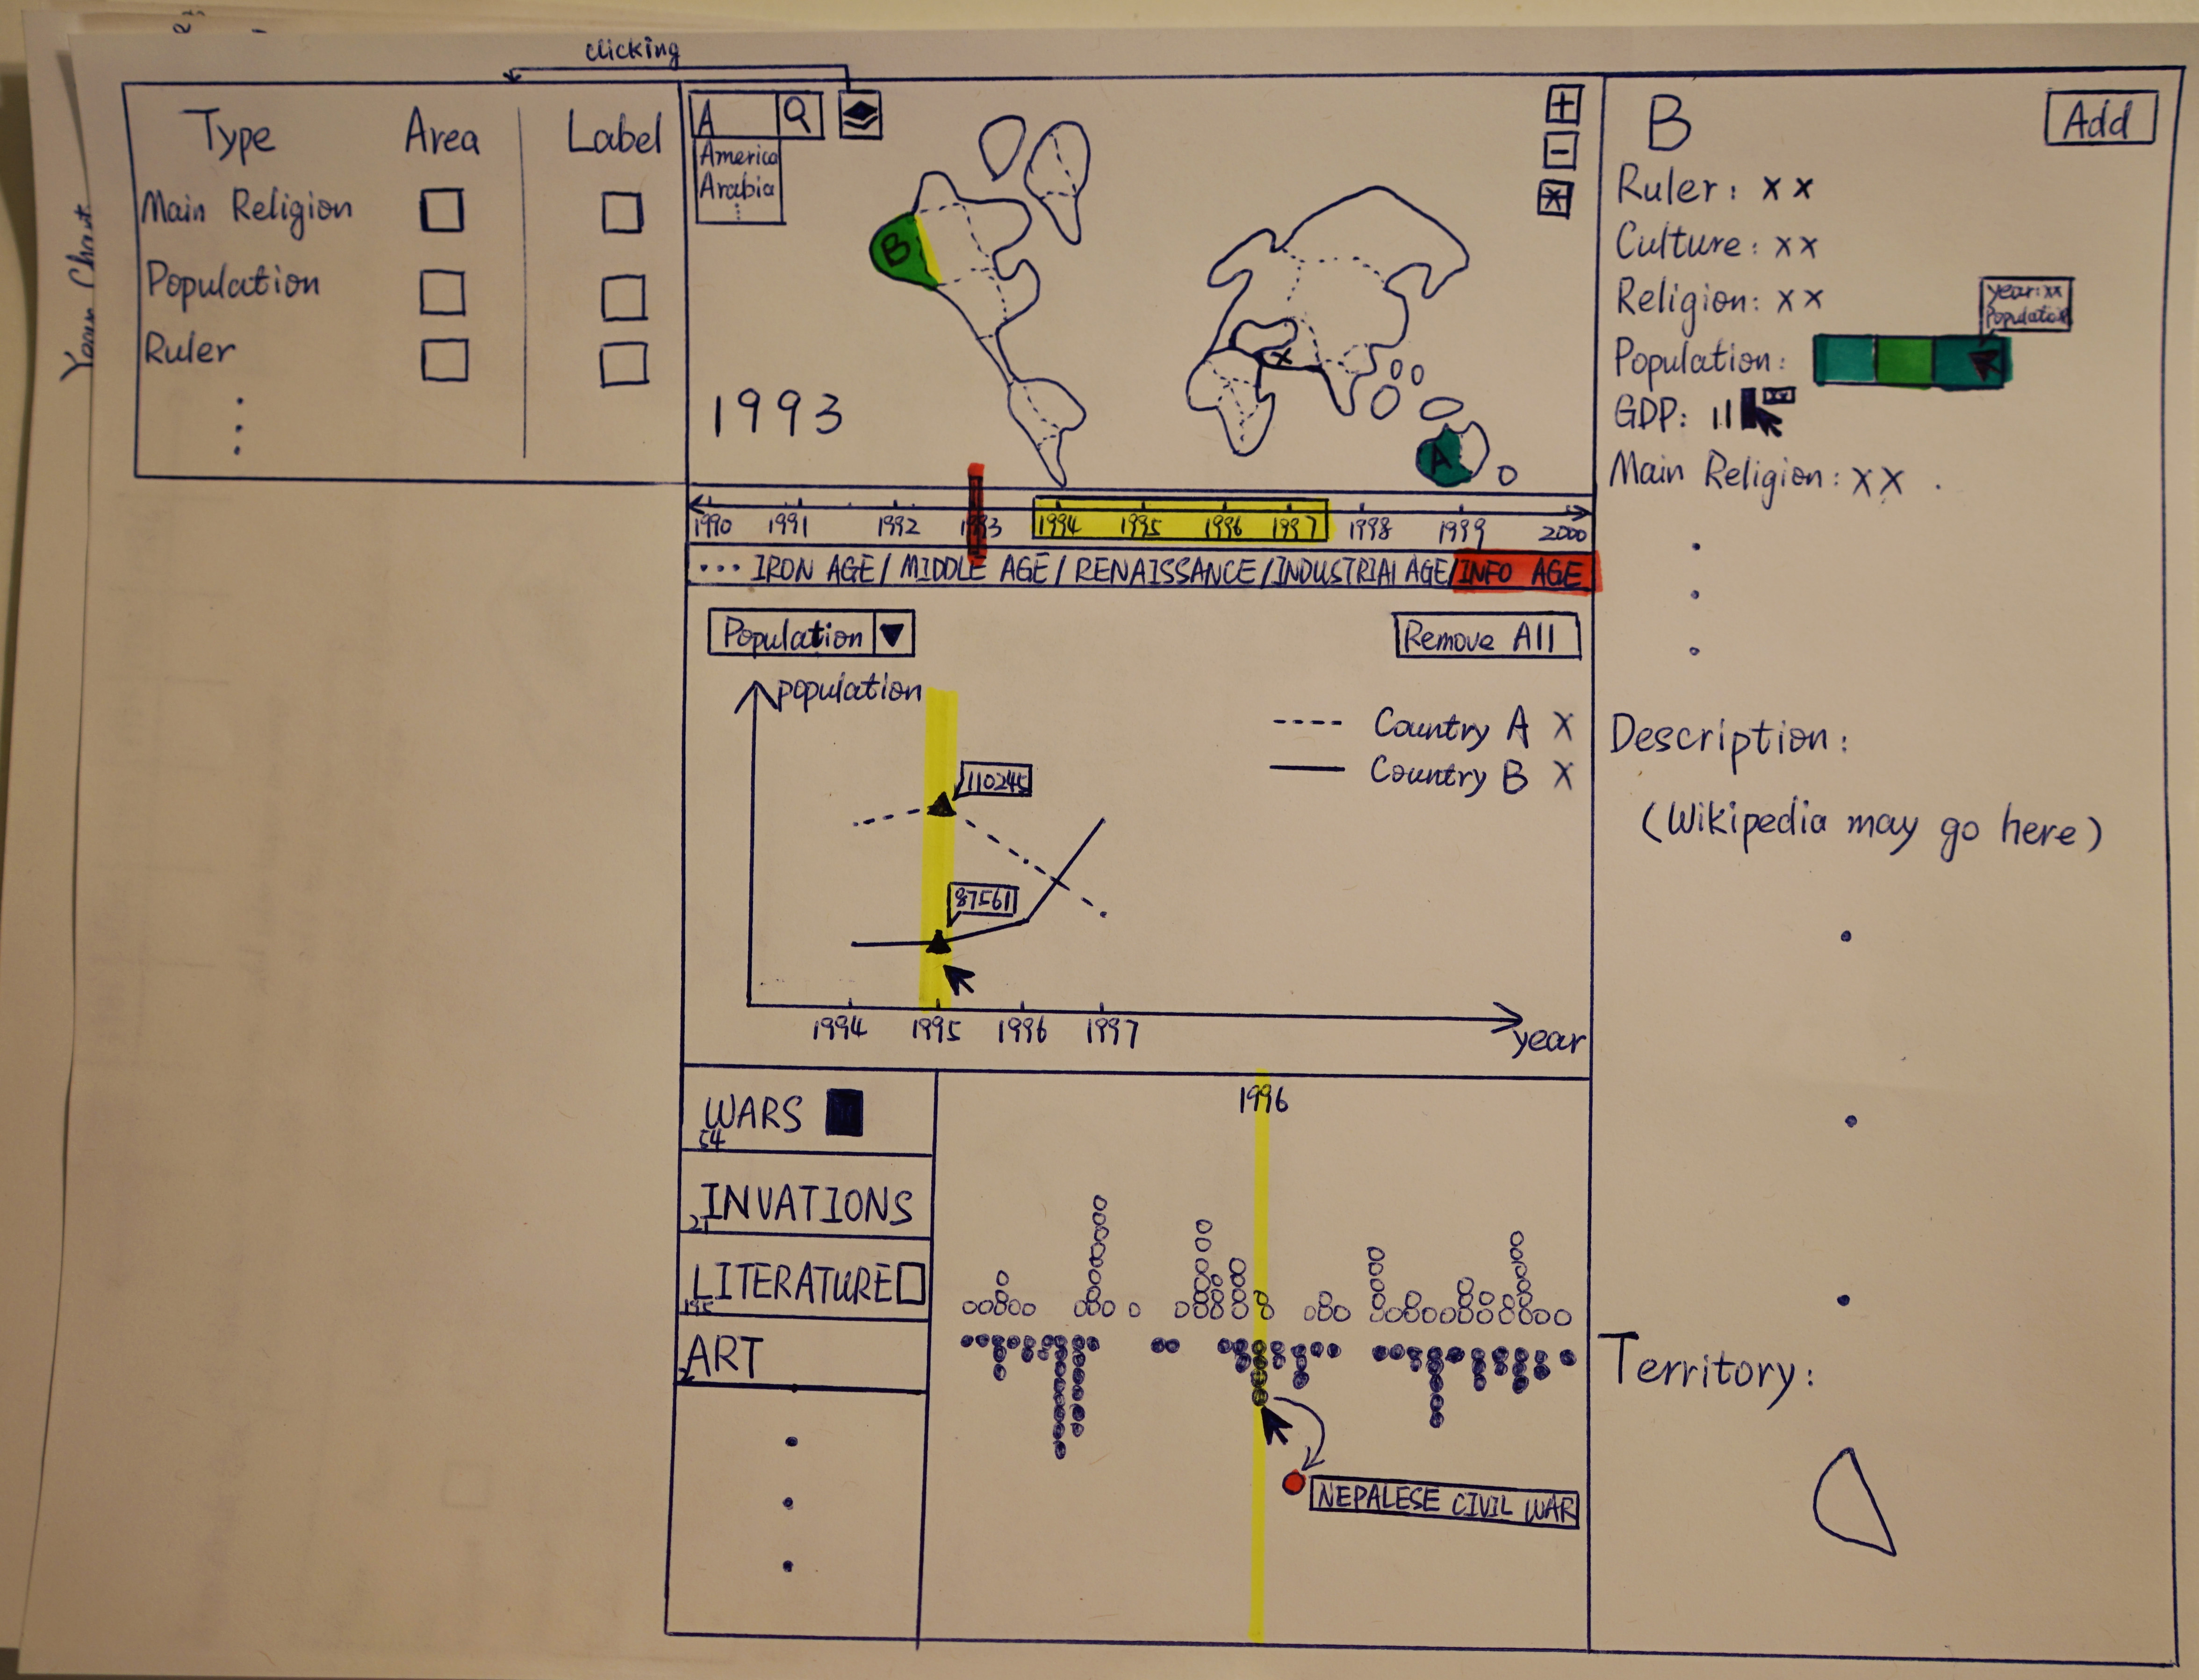
\includegraphics[width=\textwidth]{figs/original.jpg}
        \caption{Original design in our proposal.}
        \label{fig:original}
    \end{center}
\end{figure}
\newpage

\section{Implementation}
Our implementation is mostly based on d3. We also use two external plugins: DataTable and SlideBar. Our styling is based on Bootstrap 4.
\subsection{Miscellaneous}
\subsubsection{Loader}
In our project, there are a lot of data to be read before the visualization
could work, which may take several seconds.  We add a tiny spinning ring as the loader while loading
the data. After all data are loaded, the loader will disappear and the user can
start having fun with the visualizations.
The design is shown below:
\subsubsection{Header}
The header is used to switch the page to process book, screencast and about pages.
We simply use a bootstrap nav-bar component as the header.
The design is shown below:

\subsection{Map View}
Figure \ref{fig:mapoverview} is an overview of the Map View. The components are explained below:
\begin{figure}[h!]
    \begin{center}
        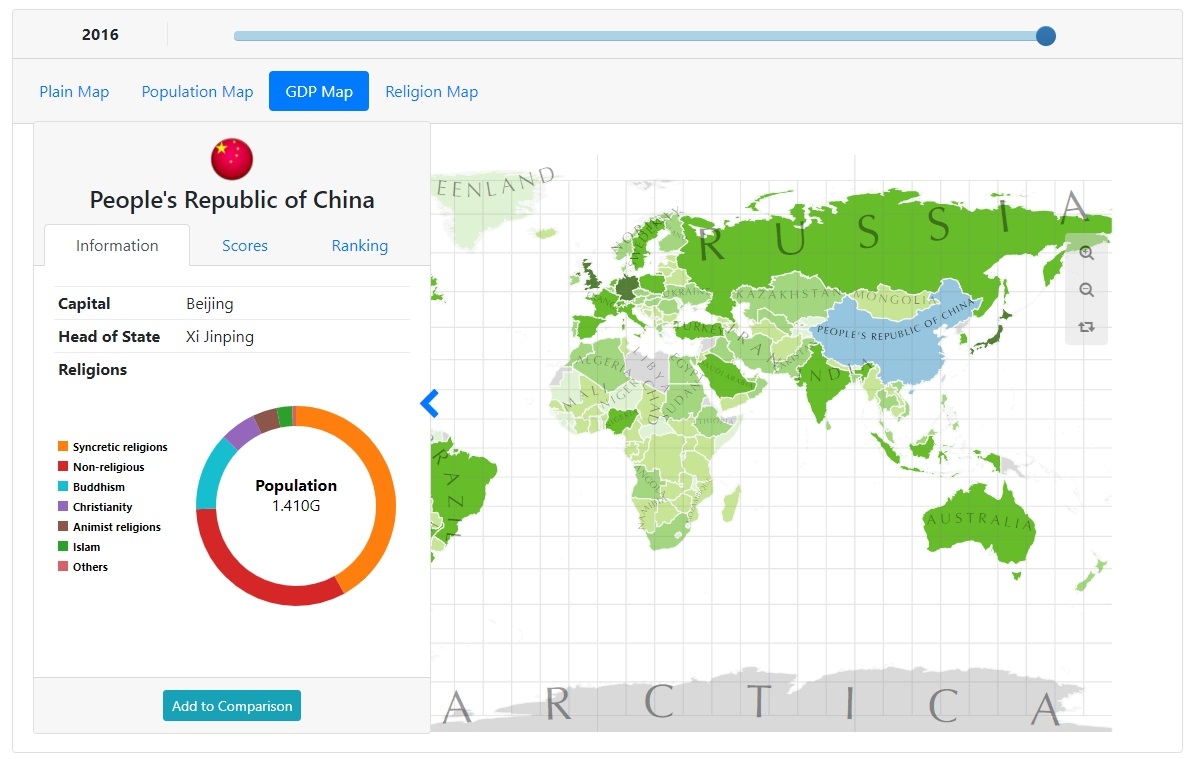
\includegraphics[width=\textwidth]{figs/mapoverview.jpg}
        \caption{An overview of Map View.}
        \label{fig:mapoverview}
    \end{center}
\end{figure}

\subsubsection{Year Selection}
We used a combination of text and slider for year selections.
The text shows the current year, and the slider is used to change the year.
They are put at the top of map view.

\subsubsection{Map}
In the map, we draw the country borders according to the GeoJSON data.
We further add zoom functionality to the country so that we can choose countries that have small areas.

The non-trivial part is the country name placement. Country names are essential in our project,
but if we just simply put the labels at the centroids, the result can be terrible (shown in Figure \ref{fig:badcnname}). We finally come up with an elegant
design (on our own!): we first decompose each country into continuous polygons, and pick the polygon with largest area (e.g. for the U.S., only the continent part will remain).
Then we calculated the longest segment within the polygon (using Rotating Calipers Algorithm), and place the label on that line.
The font size will be dynamically adjusted according to the ratio between the segment length and the label length.

When a user move mouse over a country, it will be filled with light blue. When a user click on a country, it will be filled with dark blue, and 
an information panel is shown.

The design is shown in Figure \ref{fig:ourcnname}:

\begin{figure}[h!]
    \begin{minipage}{0.49\linewidth}
        \centering
        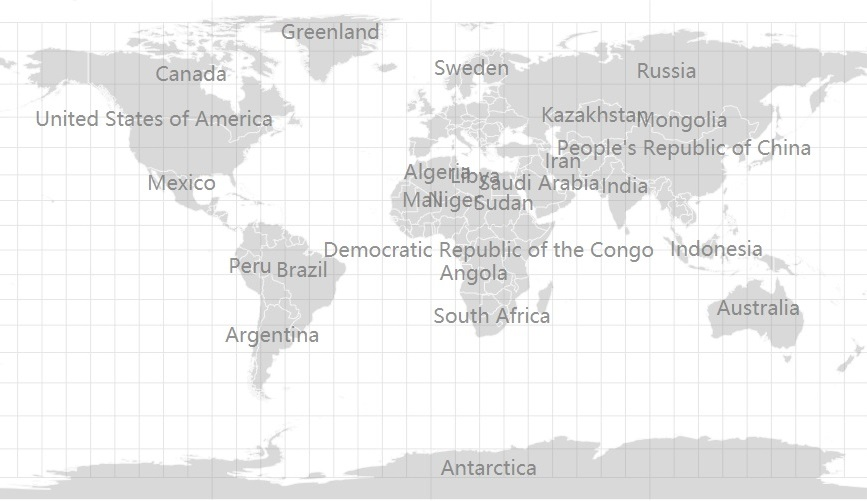
\includegraphics[width=\textwidth]{figs/badcnname.jpg}
        \caption{A bad design for country label placement.}
        \label{fig:badcnname}
    \end{minipage}
    \hfill\
    \begin{minipage}{0.49\linewidth}
        \centering
        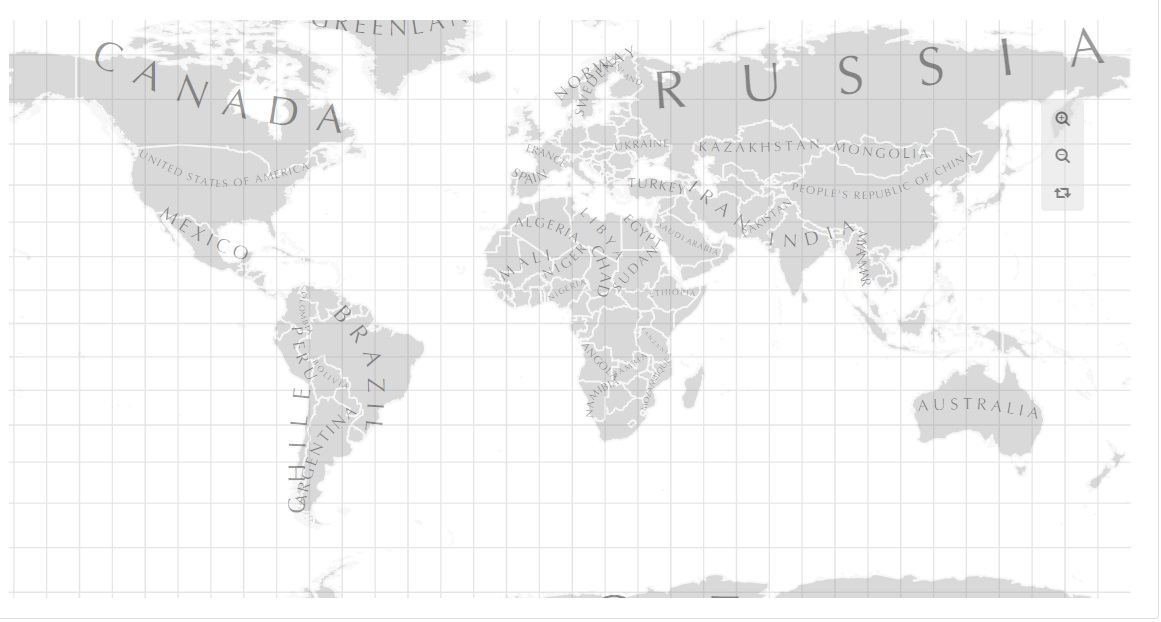
\includegraphics[width=\textwidth]{figs/map.jpg}
        \caption{Our country label placement scheme.}
        \label{fig:ourcnname}
    \end{minipage}
\end{figure} 


\subsubsection{Heat Maps}
Heat maps are good tools for us to understand the distribution of some statistics like populations.
In our project, we support three categories of heat maps: population, GDP and religion.
For population and GDP, we divide the domain into five bins, and color the countries with the corresponding bin.
For religion map, we color the countries with its major religion.
A legend for the heat map is drawn in the bottom-left corner of the map.

The design is shown in Figure \ref{fig:heatp} and \ref{fig:heatr}:
\begin{figure}[h!]
    \begin{minipage}{0.49\linewidth}
        \centering
        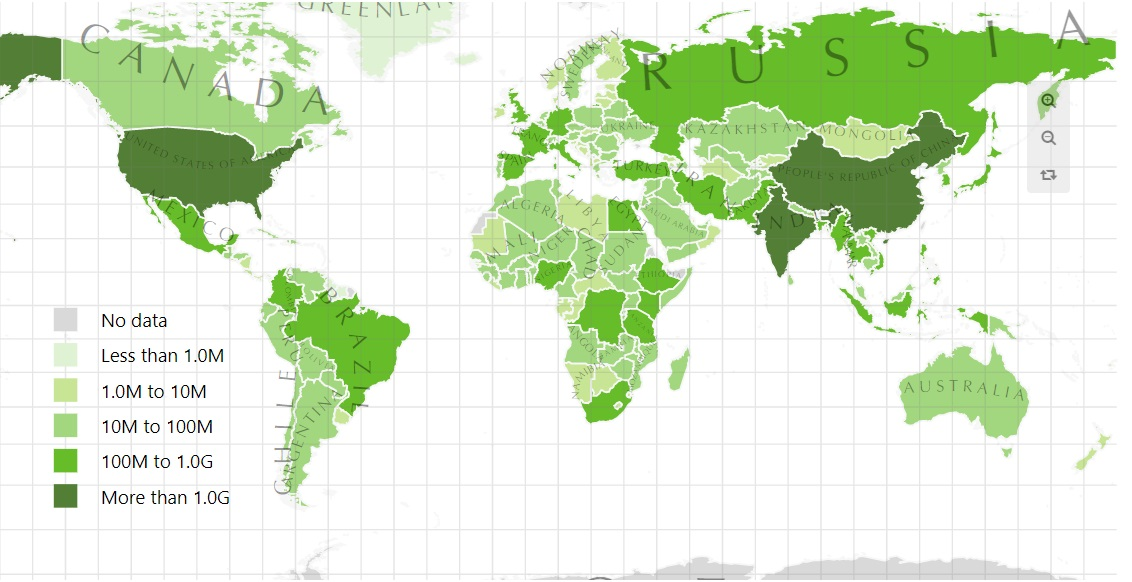
\includegraphics[width=\textwidth]{figs/heatmapp.jpg}
        \caption{Population Heat Map.}
        \label{fig:heatp}
    \end{minipage}
    \hfill\
    \begin{minipage}{0.49\linewidth}
        \centering
        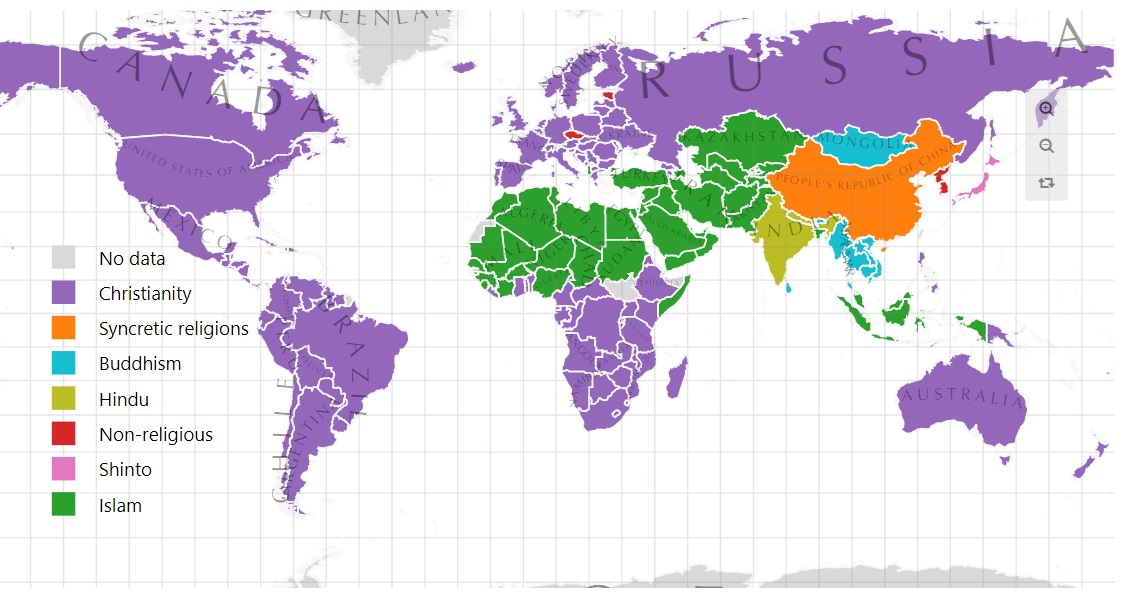
\includegraphics[width=\textwidth]{figs/heatmapr.jpg}
        \caption{Religion Heat Map.}
        \label{fig:heatr}
    \end{minipage}
\end{figure} 

\subsubsection{Information Panel}
The information panel is shown when a country is clicked. It can be collapsed and recovered freely.
There are three tabs which are information, scores and ranking.

In the information tab, we see the basic information of this country, which includes capital, head of state, population and religion information.
A donut chart is drawn to show the proportions of different religions, as well as the population of that religion.
When a user move the mouse on a sector, the sector will be enlarged and the data of the corresponding religion will be shown at the center of the donut.
The design is shown in Figure \ref{fig:info1}.

In the scores tab, we show a radar chart for five aspects of the country. The scores are normalized into range $[0,100]$. The best country has score $100$,
and other countries have score proportional to the raw data.
The design is shown in Figure \ref{fig:info2}.

In the ranking tab, we show the ranking of the country in the world. The clicked country is labeled by a marker on a area chart, which represents the data for all countries.
The detailed information is shown on mouse hovering.
The design is shown in Figure \ref{fig:info3}.

Finally, we can click the Add to Comparison button to mark the clicked country as selected.
When the country is already selected, the button become Remove from Comparison.
The Comparison View will show detailed statistics of the selected country, which will be described below.

\begin{figure}[h!]
    \begin{minipage}{0.31\linewidth}
        \centering
        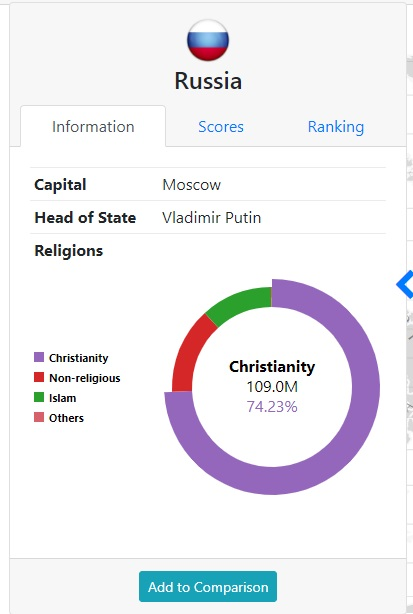
\includegraphics[width=\textwidth]{figs/info1.jpg}
        \caption{Information Tab.}
        \label{fig:info1}
    \end{minipage}
    \hfill\
    \begin{minipage}{0.31\linewidth}
        \centering
        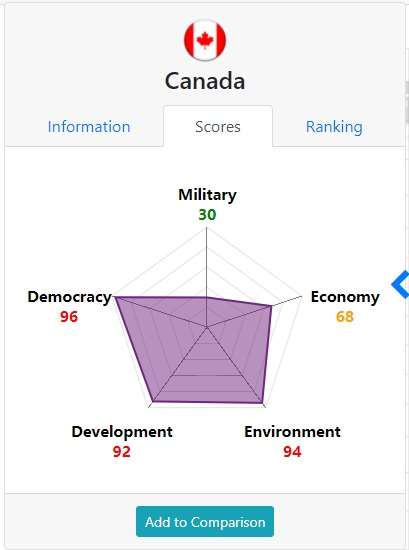
\includegraphics[width=\textwidth]{figs/info2.jpg}
        \caption{Scores Tab.}
        \label{fig:info2}
    \end{minipage}
    \hfill\
    \begin{minipage}{0.31\linewidth}
        \centering
        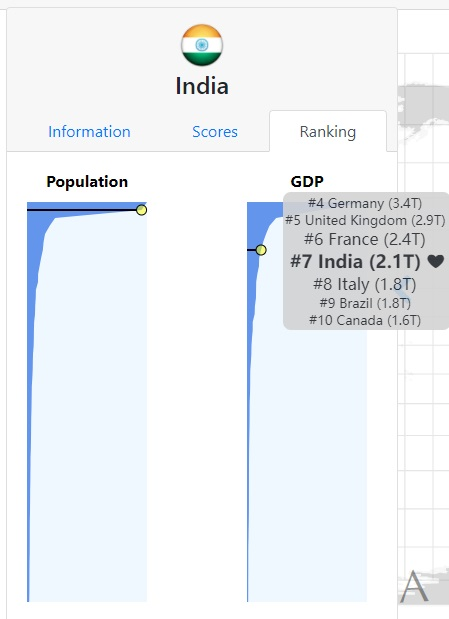
\includegraphics[width=\textwidth]{figs/info3.jpg}
        \caption{Ranking Tab.}
        \label{fig:info3}
    \end{minipage}
\end{figure} 

\subsection{Comparison View}
The Comparison View shows comparison between selected country. Figure \ref{fig:cvoverview} shows an overview of Comparison View. If no country is selected,
a banner will appear to ask the user to select at least one country.

\begin{figure}[h!]
    \begin{center}
        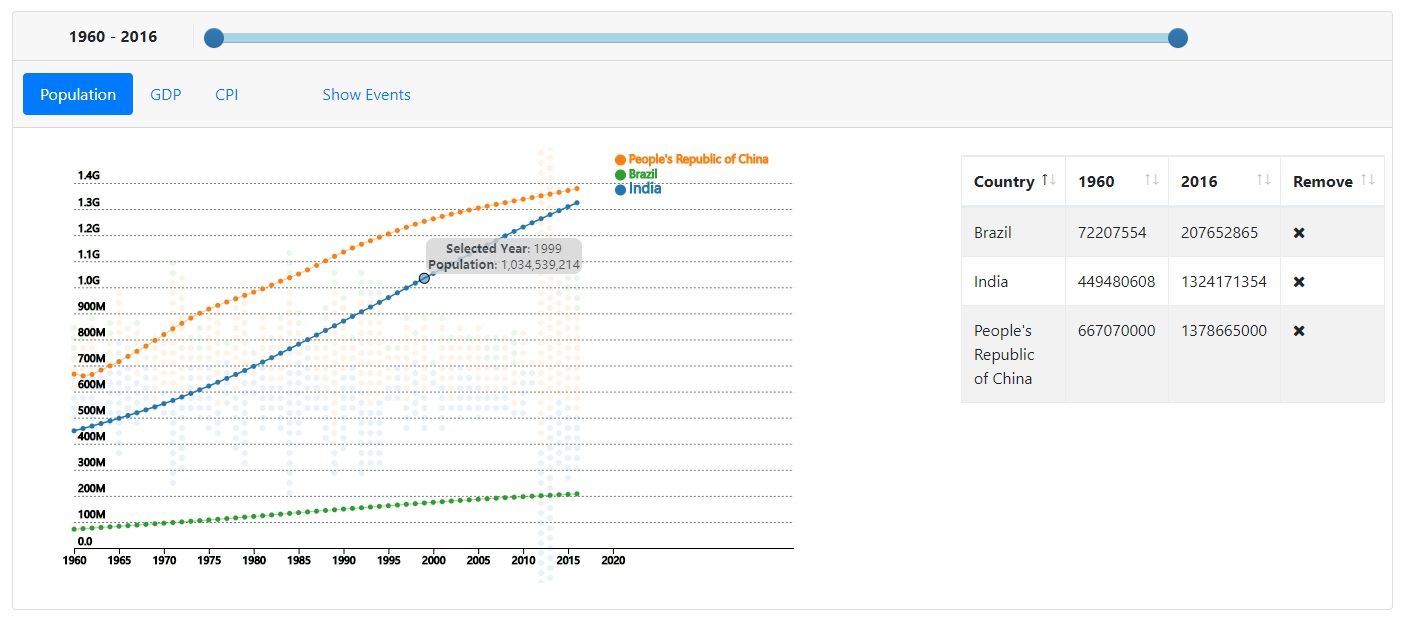
\includegraphics[width=\textwidth]{figs/cvoverview.jpg}
        \caption{An overview of Comparison View.}
        \label{fig:cvoverview}
    \end{center}
\end{figure}

\subsubsection{Range Selection}
Similar to year selection, we also use a combination of text and slider to choose the range of years.
The only difference is that now the slider contains two circles so that we can select a range.

\subsubsection{Data Table}
The data tables contains the data of selected countries at the two ends of the year range.
We can sort them accordingly.
We use the DataTable plugin to construct the table.
The design is shown in \ref{fig:datatable}.

\subsubsection{Line Charts}

The data are illustrated by line charts. Each country is assigned with one color for the line and the points.
A tip containing the values will shown on mouse hovering, as shown in Figure \ref{fig:cvoverview}.
Besides, a user can temporarily hide the data for a country by clicking its legend, and add it back by clicking again.
Figure \ref{fig:hideline} shows an example for that.

\begin{figure}[h!]
    \begin{center}
        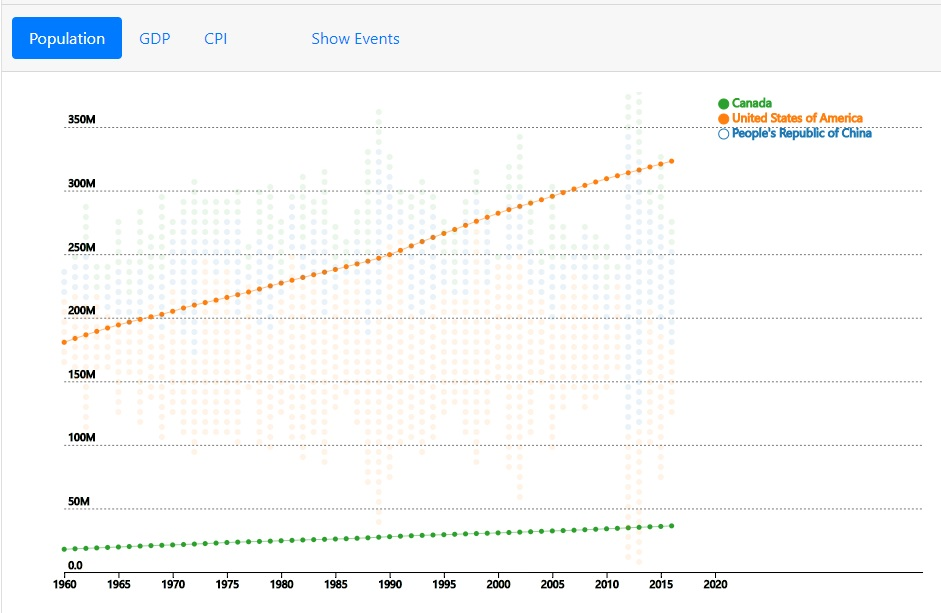
\includegraphics[width=\textwidth]{figs/hideline.jpg}
        \caption{An example of temporarily removing a country.}
        \label{fig:hideline}
    \end{center}
\end{figure}
\subsubsection{Events}

Finally, the Show Events button shows the events above the line chart.
The events are represented by circles filled by color representing related country.
They are placed according to their times. A tip containing detailed information will shown on mouse hovering.
With the events we can exploit the causality behind historical trends.
The design is shown in \ref{fig:events}.

\begin{figure}[h!]
    \begin{minipage}{0.49\linewidth}
        \centering
        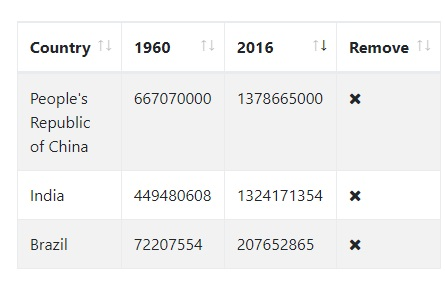
\includegraphics[width=\textwidth]{figs/datatable.jpg}
        \caption{An example of sorting data on data table.}
        \label{fig:datatable}
    \end{minipage}
    \hfill\
    \begin{minipage}{0.49\linewidth}
        \centering
        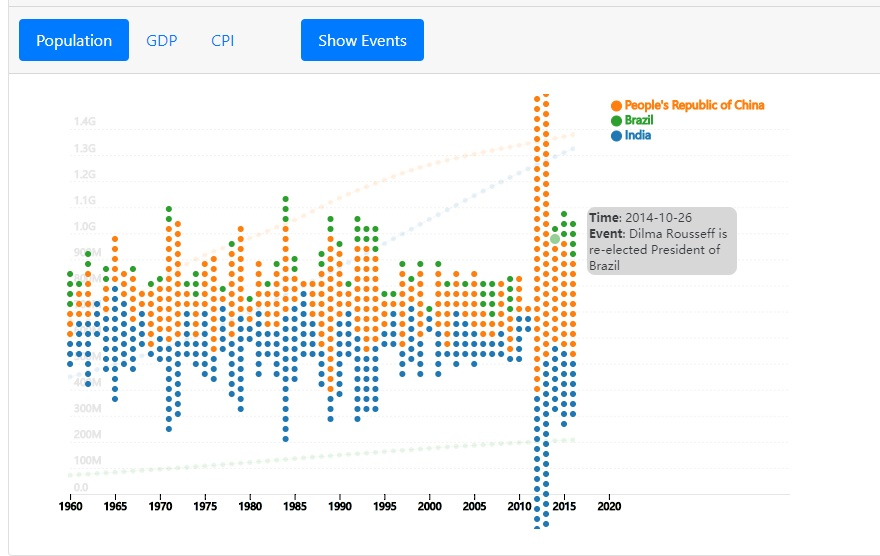
\includegraphics[width=\textwidth]{figs/events.jpg}
        \caption{Showing events.}
        \label{fig:events}
    \end{minipage}
\end{figure} 

\section{Evaluation}
In our point of view, our project successfully achieve the objectives:
\begin{itemize}
    \item Historical world map is shown in the map view.

    \item The basic information and religious composition of a country is shown in the information panel.

    \item The comparison on different aspects of a country is shown in the Score tab in the information panel.

    \item The rankings of a country are shown in the the Ranking tab in the information panel.

    \item The population/GDP/religion distribution of the world is shown in the heatmaps.

    \item The historical statistics of a country is shown in the comparison view.

    \item Comparison between different countries is shown in the comparison view.

    \item The relation between historical events and statistics trends are reflected by the comparison view.
\end{itemize}

However, due to the time limitation, this project is far from project. We would like to improve it in the following ways:
\begin{itemize}
    \item Include more datasets.
    \item Add a search functionality so that we can select a country that we don't know its location.
    \item Add smart selection functionality so that we can compare a country with, say, all countries that are in the same area.
\end{itemize}

\end{document}
